\documentclass{article}\usepackage[]{graphicx}\usepackage[]{xcolor}
% maxwidth is the original width if it is less than linewidth
% otherwise use linewidth (to make sure the graphics do not exceed the margin)
\makeatletter
\def\maxwidth{ %
  \ifdim\Gin@nat@width>\linewidth
    \linewidth
  \else
    \Gin@nat@width
  \fi
}
\makeatother

\definecolor{fgcolor}{rgb}{0.345, 0.345, 0.345}
\newcommand{\hlnum}[1]{\textcolor[rgb]{0.686,0.059,0.569}{#1}}%
\newcommand{\hlsng}[1]{\textcolor[rgb]{0.192,0.494,0.8}{#1}}%
\newcommand{\hlcom}[1]{\textcolor[rgb]{0.678,0.584,0.686}{\textit{#1}}}%
\newcommand{\hlopt}[1]{\textcolor[rgb]{0,0,0}{#1}}%
\newcommand{\hldef}[1]{\textcolor[rgb]{0.345,0.345,0.345}{#1}}%
\newcommand{\hlkwa}[1]{\textcolor[rgb]{0.161,0.373,0.58}{\textbf{#1}}}%
\newcommand{\hlkwb}[1]{\textcolor[rgb]{0.69,0.353,0.396}{#1}}%
\newcommand{\hlkwc}[1]{\textcolor[rgb]{0.333,0.667,0.333}{#1}}%
\newcommand{\hlkwd}[1]{\textcolor[rgb]{0.737,0.353,0.396}{\textbf{#1}}}%
\let\hlipl\hlkwb

\usepackage{framed}
\makeatletter
\newenvironment{kframe}{%
 \def\at@end@of@kframe{}%
 \ifinner\ifhmode%
  \def\at@end@of@kframe{\end{minipage}}%
  \begin{minipage}{\columnwidth}%
 \fi\fi%
 \def\FrameCommand##1{\hskip\@totalleftmargin \hskip-\fboxsep
 \colorbox{shadecolor}{##1}\hskip-\fboxsep
     % There is no \\@totalrightmargin, so:
     \hskip-\linewidth \hskip-\@totalleftmargin \hskip\columnwidth}%
 \MakeFramed {\advance\hsize-\width
   \@totalleftmargin\z@ \linewidth\hsize
   \@setminipage}}%
 {\par\unskip\endMakeFramed%
 \at@end@of@kframe}
\makeatother

\definecolor{shadecolor}{rgb}{.97, .97, .97}
\definecolor{messagecolor}{rgb}{0, 0, 0}
\definecolor{warningcolor}{rgb}{1, 0, 1}
\definecolor{errorcolor}{rgb}{1, 0, 0}
\newenvironment{knitrout}{}{} % an empty environment to be redefined in TeX

\usepackage{alltt}
\usepackage{amsmath} %This allows me to use the align functionality.
                     %If you find yourself trying to replicate
                     %something you found online, ensure you're
                     %loading the necessary packages!
\usepackage{amsfonts}%Math font
\usepackage{graphicx}%For including graphics
\usepackage{hyperref}%For Hyperlinks
\usepackage[shortlabels]{enumitem}% For enumerated lists with labels specified
                                  % We had to run tlmgr_install("enumitem") in R
\hypersetup{colorlinks = true,citecolor=black} %set citations to have black (not green) color
\usepackage{natbib}        %For the bibliography
\setlength{\bibsep}{0pt plus 0.3ex}
\bibliographystyle{apalike}%For the bibliography
\usepackage[margin=0.50in]{geometry}
\usepackage{float}
\usepackage{multicol}

%fix for figures
\usepackage{caption}
\newenvironment{Figure}
  {\par\medskip\noindent\minipage{\linewidth}}
  {\endminipage\par\medskip}
\IfFileExists{upquote.sty}{\usepackage{upquote}}{}
\begin{document}

\vspace{-1in}
\title{Lab 10 -- MATH 240 -- Computational Statistics}

\author{
  Yuliia Heleveria \\
  MATH 240  \\
  Colgate University  \\
  {\tt yheleveria@colgate.edu}
}

\date{02/08/2025}

\maketitle

\begin{multicols}{2}
\raggedcolumns % If your spacing gets messed up try uncommenting 
                % this line
\begin{abstract}
We investigate the relationship between sample size and margin of error in opinion polls, testing Gallup's claim that doubling the sample size cuts the margin of error in half. Using simulations and resampling, we estimated margins of error and compared them with Gallup's estimates. We further examined how varying sample sizes and population proportions affect error, applying both simulation and Wilson margin of error formula. Our results show that Gallup oversimplifies the relationship between sample size and its effect on the margin of error: the margin of error depends significantly on population proportion, and doubling sample size does not reduce the margin of error by half.
\end{abstract}

\noindent \textbf{Keywords:} Margin of Error; Sample Size; Simulation; Resampling.

\section{Introduction} 

Gallup polls published a document called ``\textit{How Are Polls Conducted}'' that describes how Gallup selects people to include in its polls. In the article, Gallup claimed that with a sample size of 1,000 national adults (derived with random selection procedures), the results are likely to be accurate within a margin of error of  $\pm$4 \%. Gallup also concluded that if they increase a poll sample size to 2,000, the results then will be accurate within $\pm$2 \% of the underlying population value. 

In this lab, we tested if doubling the sample size, as Gallup claims, would reduce the margin of error in half. We performed basic simulation and resampling of a poll to test how modifying sample size would affect the margin of error. Also, we varied the population proportion to see if it would affect the margin of error.

Section \ref{sec:methods} defines methodologies. Section \ref{sec:results} presents our findings. Section \ref{sec:discussion} discusses the implications of the results and compares our findings to the Gallup's claims.



\section{Methods}\label{sec:methods}
We assume that the margin of error is based on 95\% confidence. As a example study, we chose to replicate results of February 3-16, 2025 poll of 1,004 U.S. adults about their satisfaction with position of the United States in the world today. The results revealed that 39\% of respondents were satisfied, 59\% were dissatisfied, and 2\% had no opinion. Gallup reported margin of error of $\pm$4\% for this poll.

We simulated 10,000 polls with assumed population probability proportion $p=0.39$ for sample sizes $n=1,004$ and $n=2,008$, estimating the margin of error as half the range of the middle 95\% of sample proportions. We generated 10k polls for each sample size. Simulations were created in \texttt{R} using \texttt{tidyverse}, with visualizations created using \texttt{ggplot2} and \texttt{patchwork} packages \citep{tidyverse, ggplot, patchwork}.

\begin{Figure} 
 \centering
 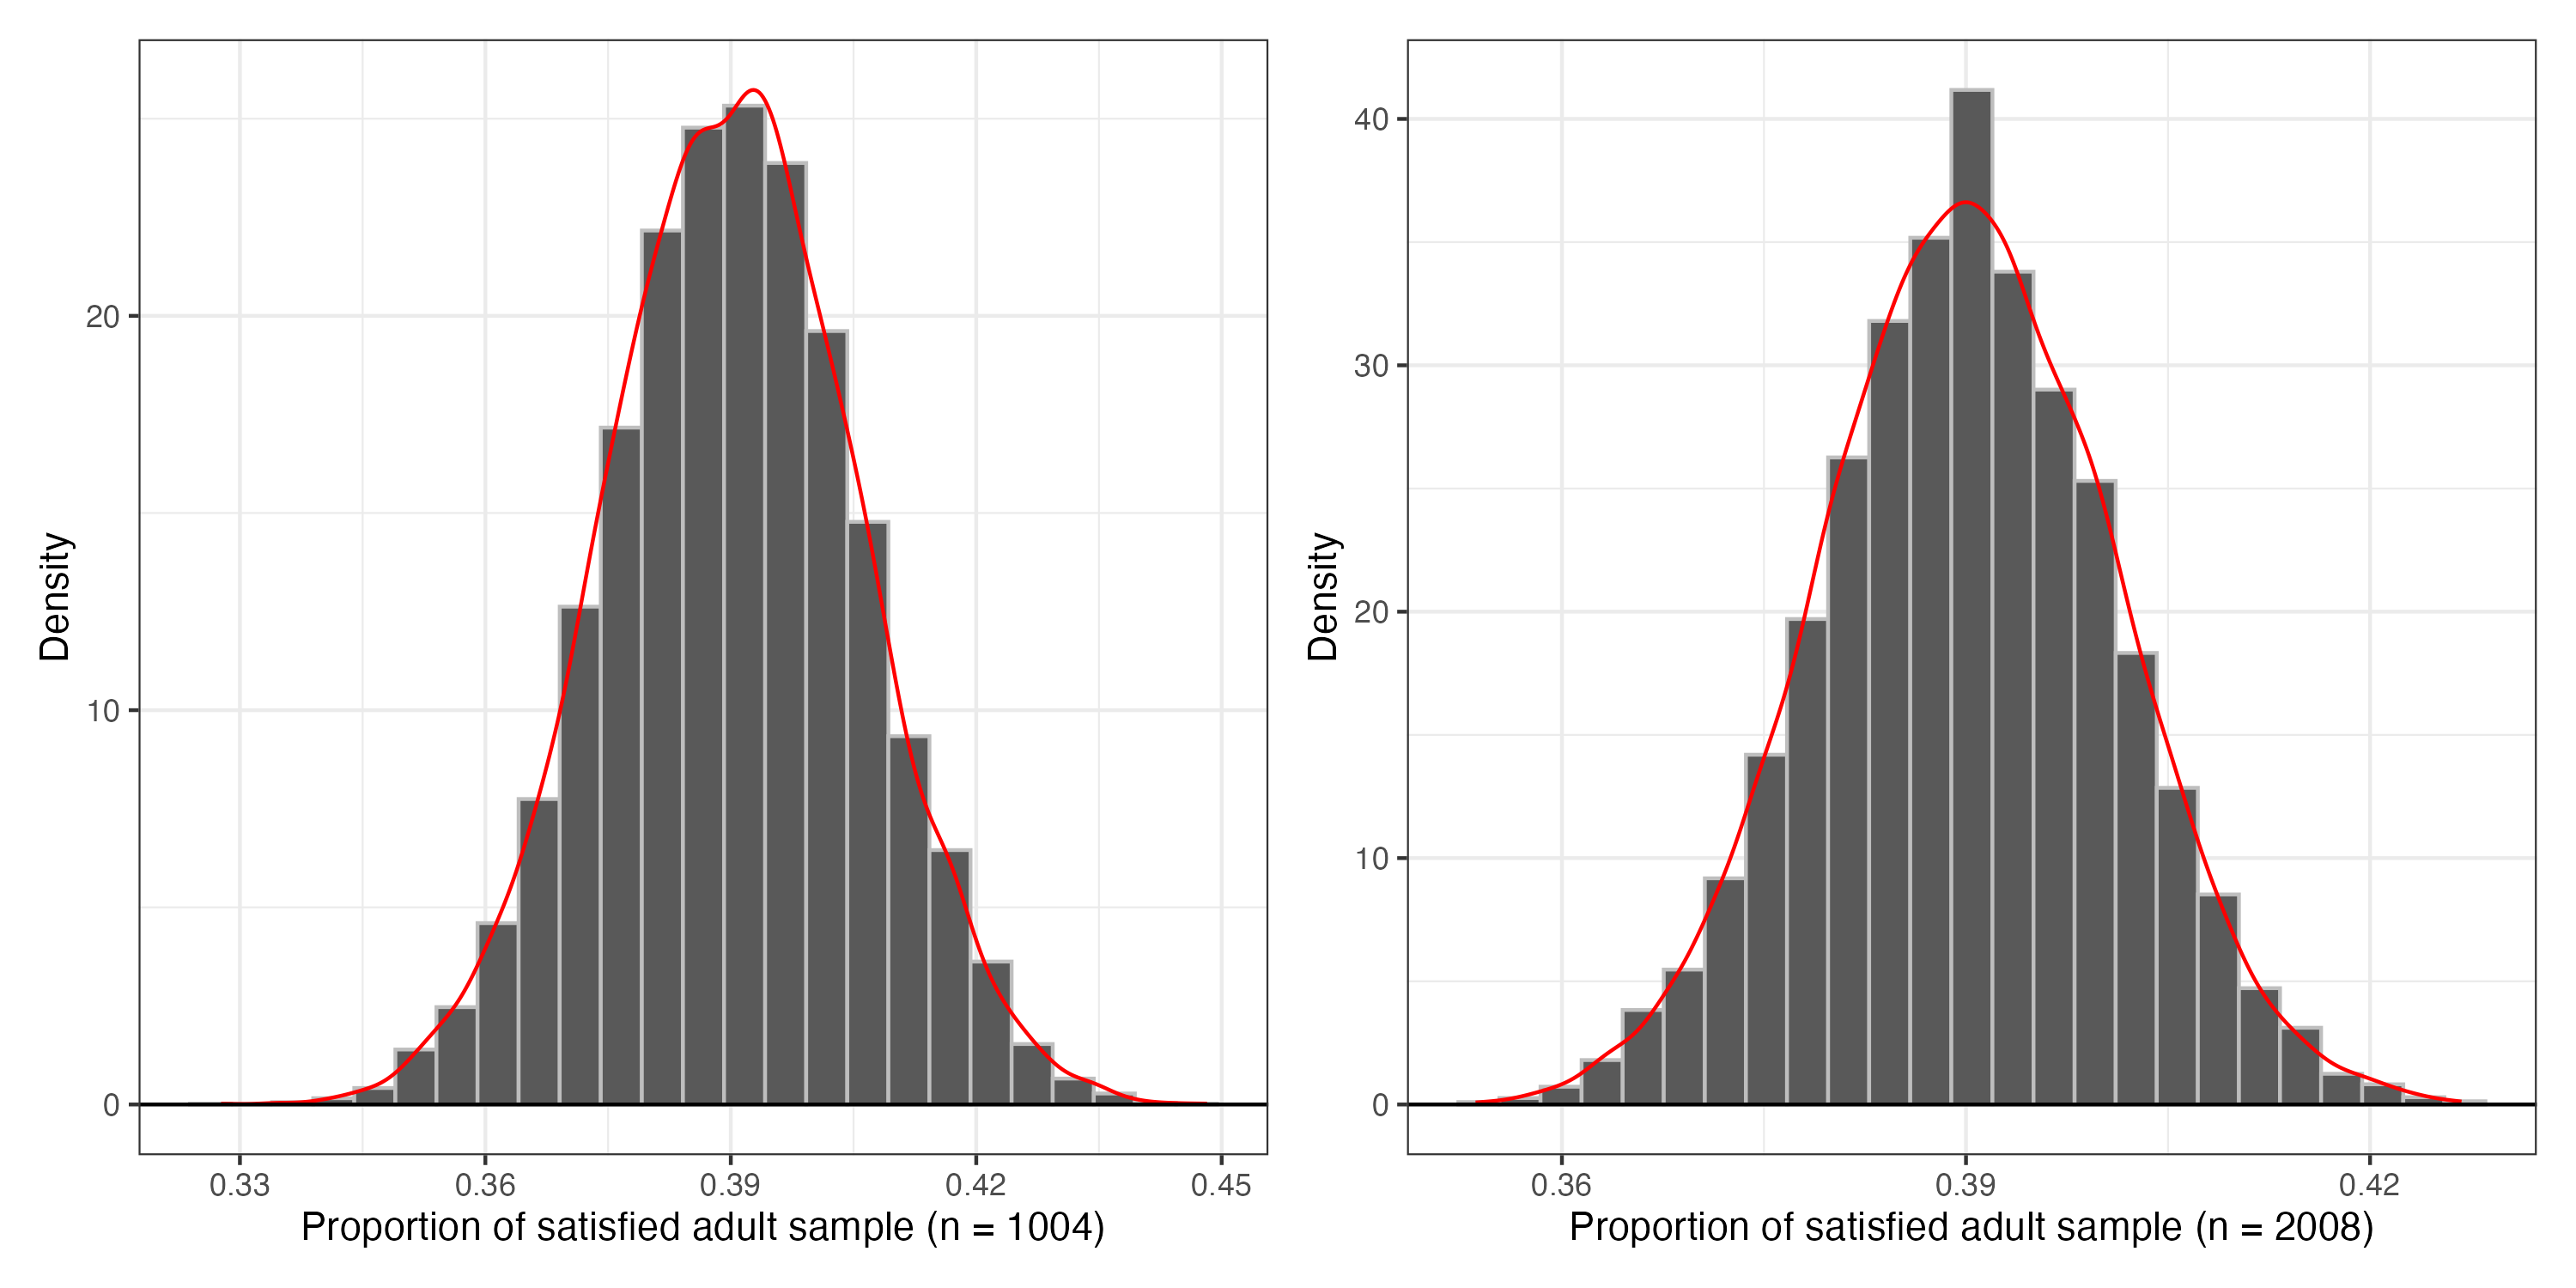
\includegraphics[width=\linewidth]{simulation.png}
 \captionof{figure}{Histogram of sample proportions with superimposed density}
 \label{fig:sim}
\end{Figure}

We also approximated the margin of error by resampling. We took random sample with replacement from the original sample 1,000 times. For each random sample taken from the original, we calculated the mean. We then summarized the range of the middle 95\% of mean values, calculating the margin of error by reducing the interval in half.

\begin{Figure}
 \centering
 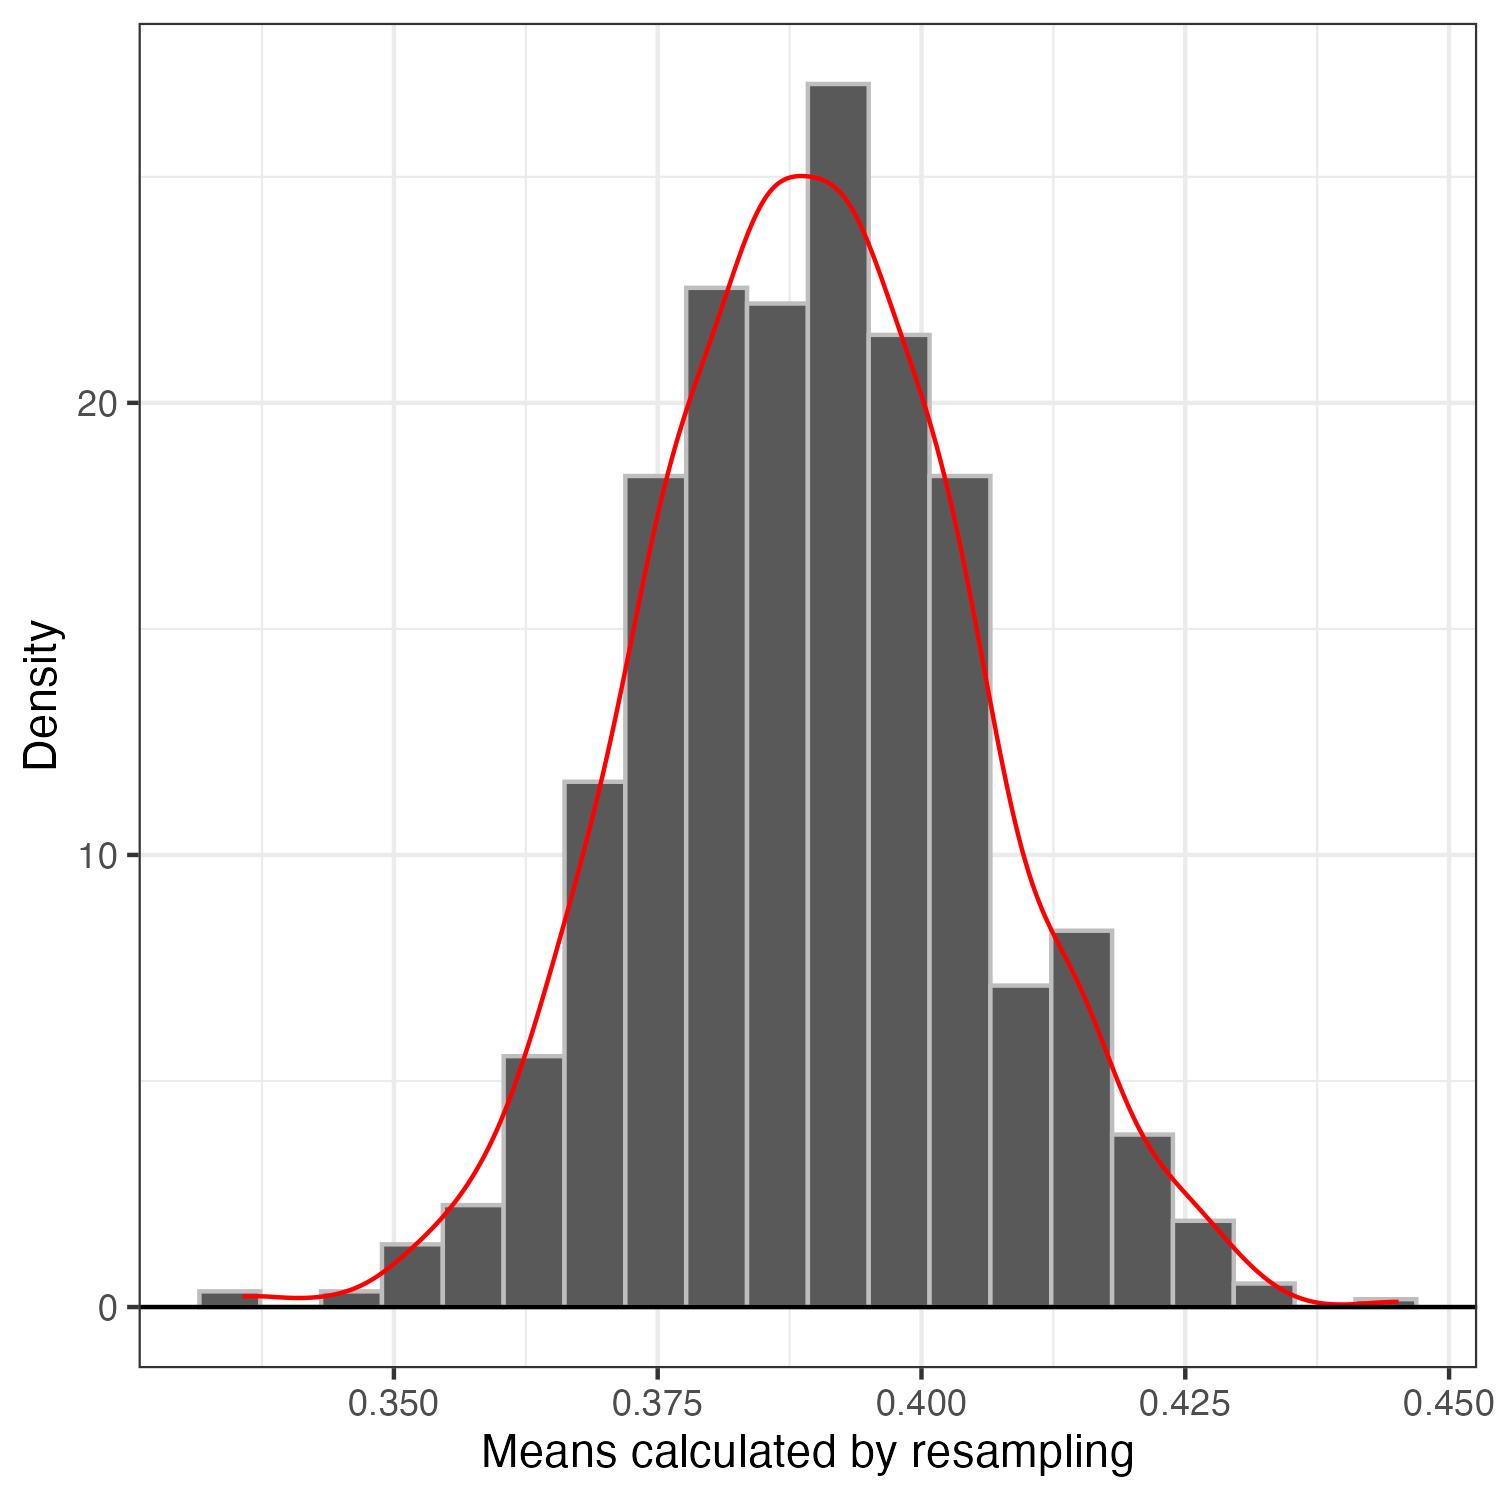
\includegraphics[width = 0.5\linewidth]{resample.png}
 \captionof{figure}{Histogram of resample proportions with superimposed density}
 \label{fig:res}
\end{Figure}

We also performed simulations for sample size $n$ in the range \{100, 110, 120, ..., 3000\} and the population probability proportion $p$ in the range \{0.01, 0.02, ..., 0.99\}. We calculated the margin of error by reducing the interval of the middle 95\% of observations in half and by using the Wilson margin of error formula.

\begin{Figure}
 \centering
 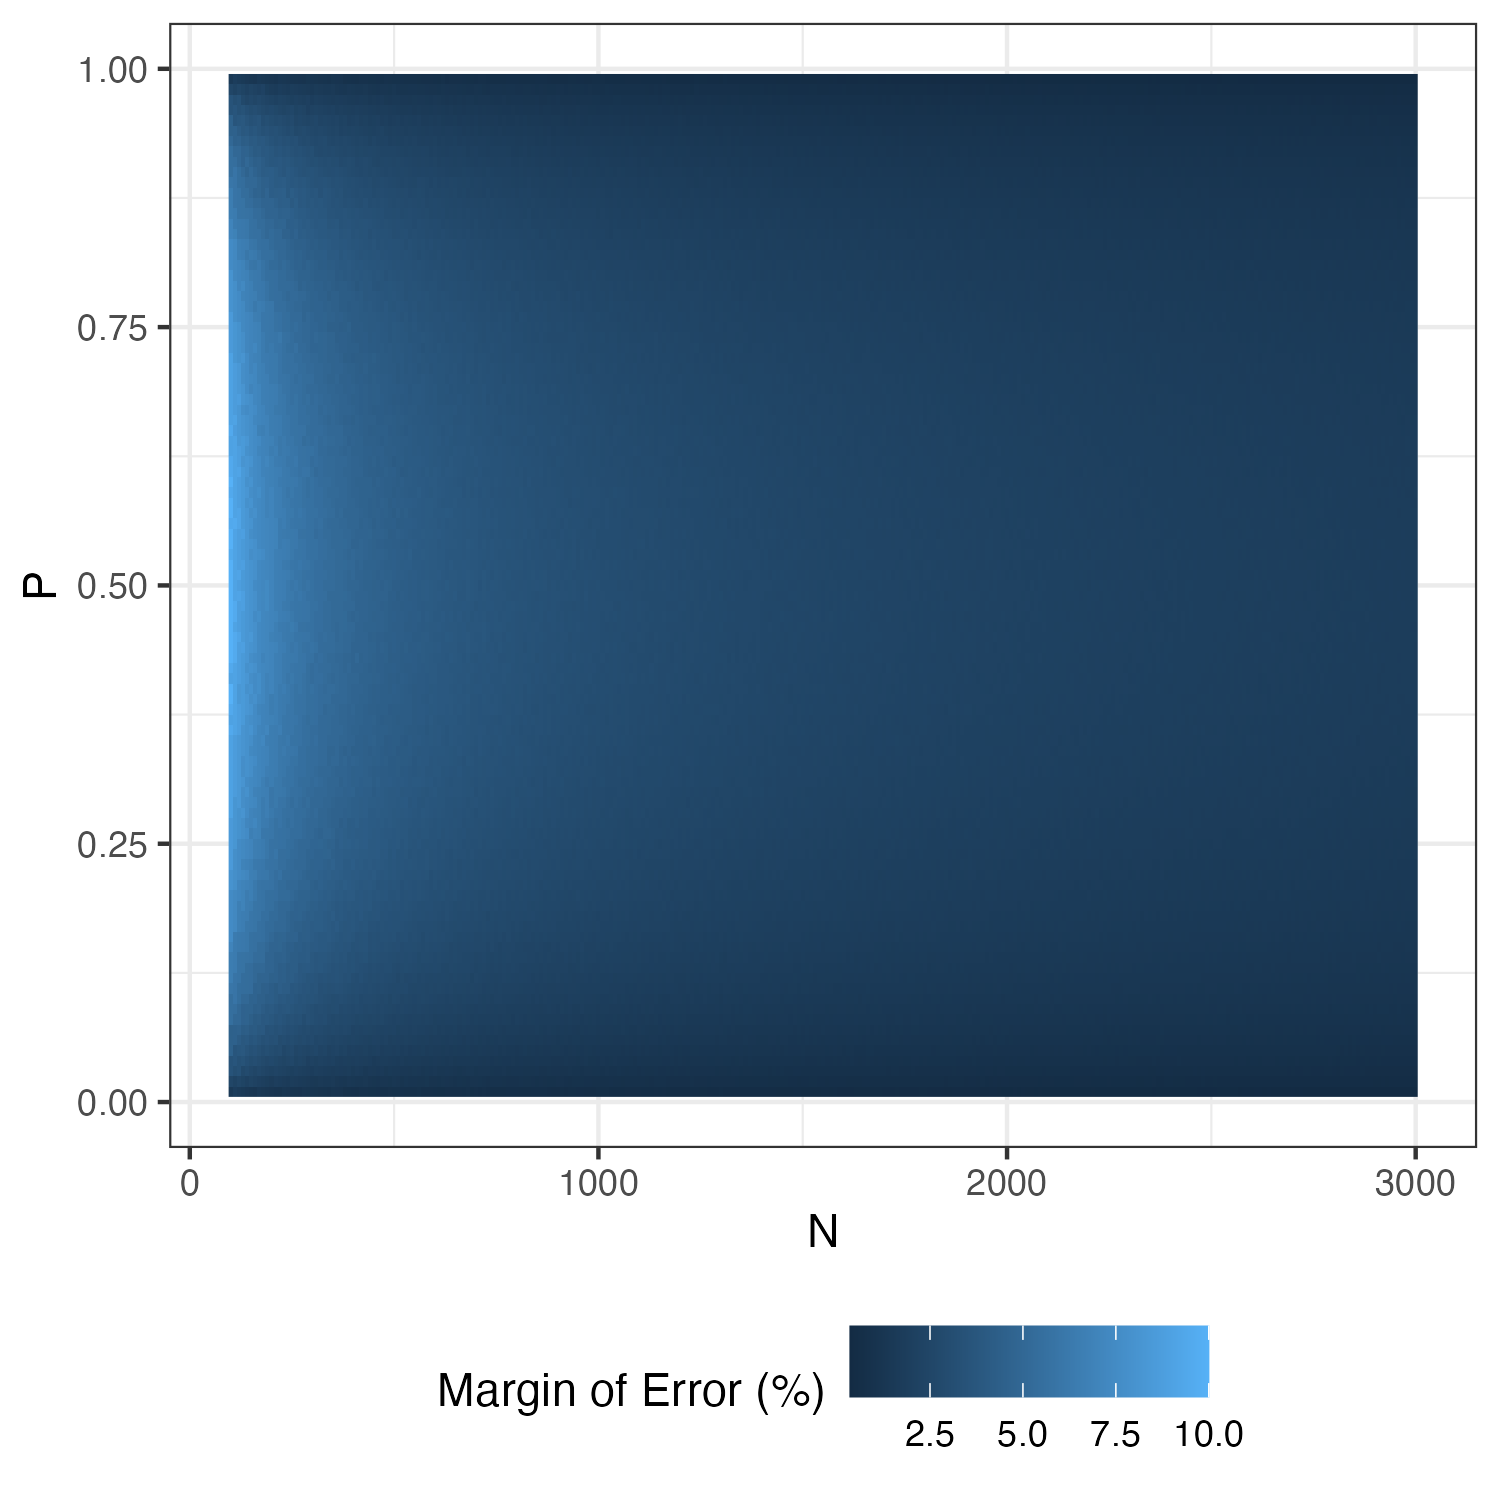
\includegraphics[width =0.7\linewidth]{error.png}
 \captionof{figure}{Estimated margin of error as a function of $n$ and $p$}
 \label{fig:err}
\end{Figure}

\begin{Figure}
 \centering
 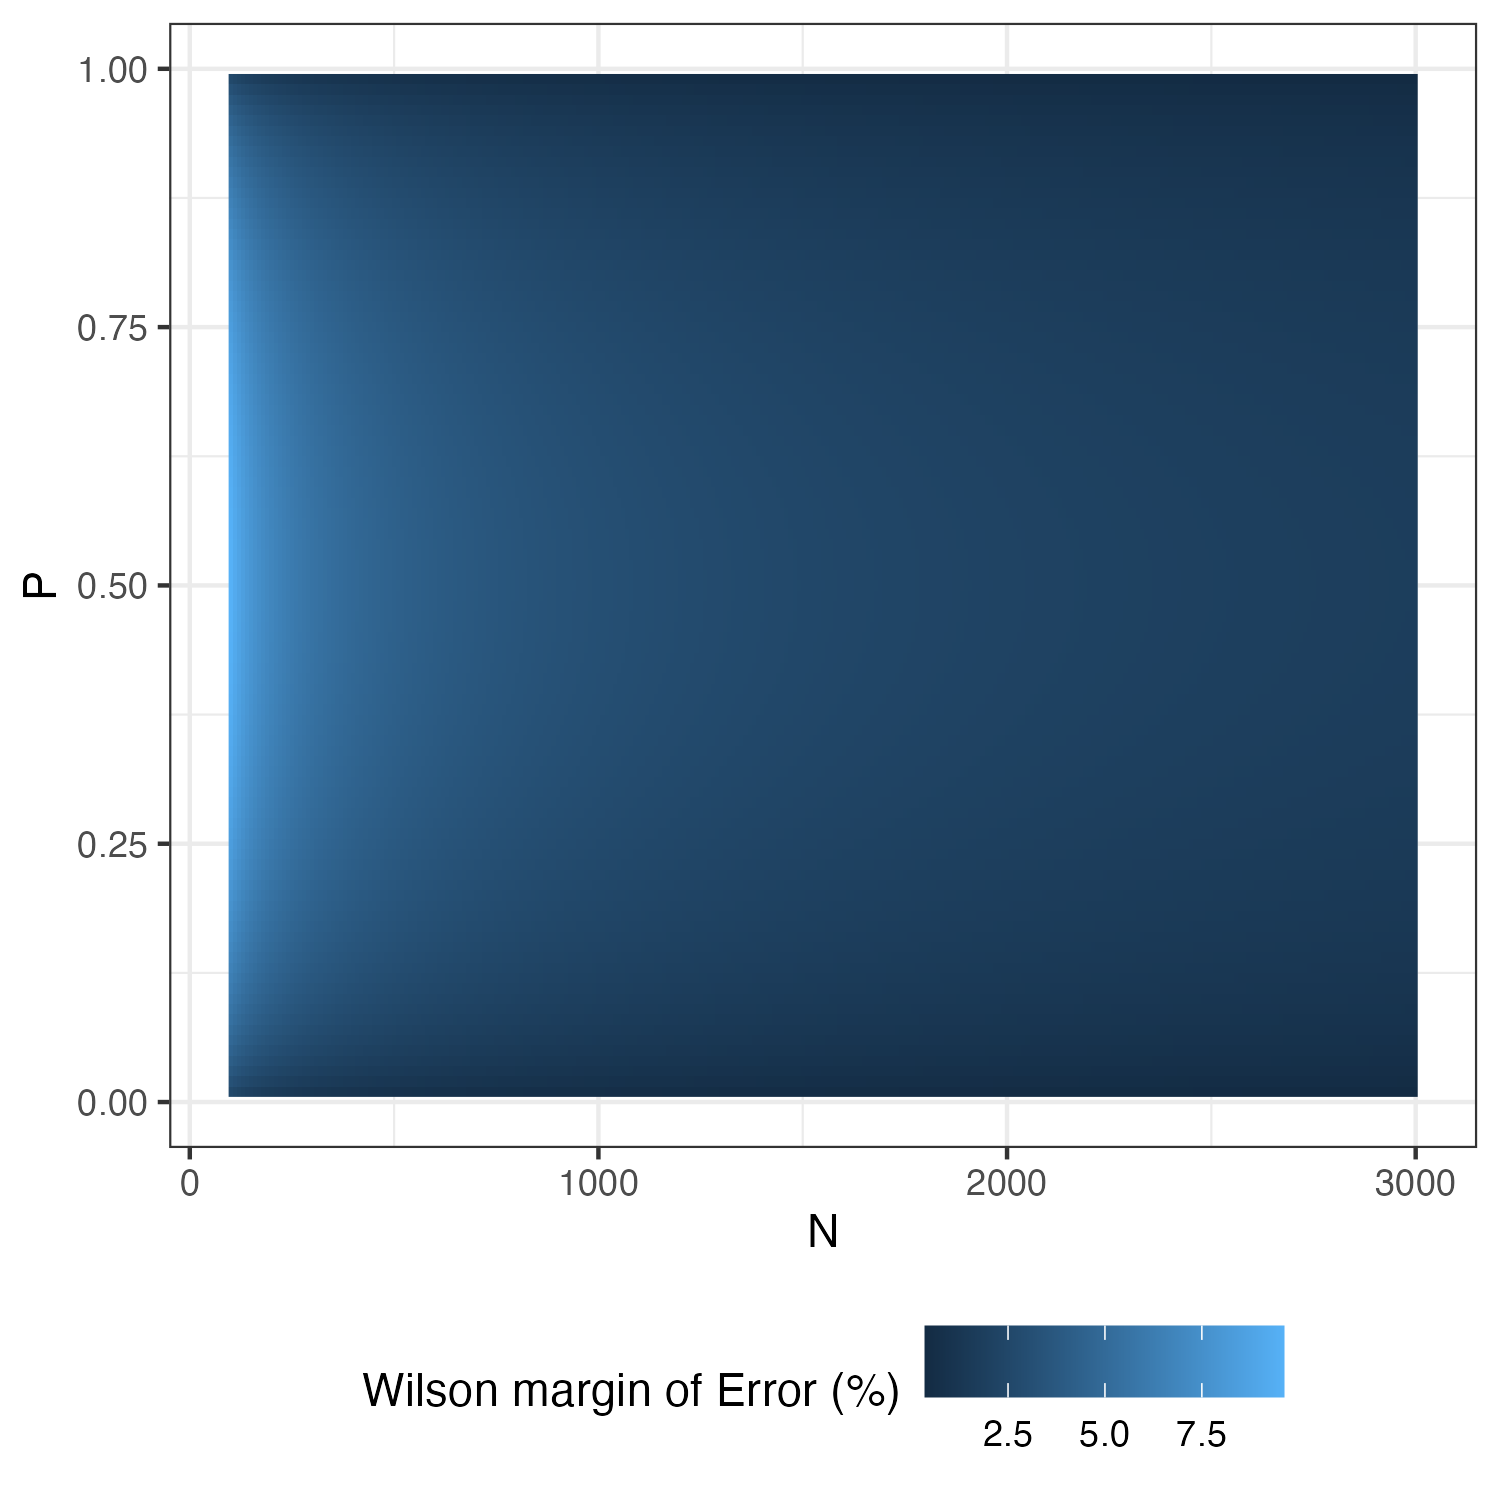
\includegraphics[width =0.7\linewidth]{error.wilson.png}
 \captionof{figure}{Wilson margin of error as a function of $n$ and $p$}
 \label{fig:errw}
\end{Figure}


\section{Results}\label{sec:results}

After we performed the basic simulation (see Figure \ref{fig:sim}), the margin of error for the sample size of 1,004 was approximately 3.04\%, which is smaller than the margin of error reported by Gallup. After we doubled the sample size to 2,008 in the simple simulation, the margin of error became approximately 2.12\%. This simple simulation does not support the Gallup's claim that the margin of error reduces in half as the sample size increases in half because our margin of error only decreased by approximately 30\%. 

The result of resampling (see Figure \ref{fig:res}) showed that the estimated margin of error for the sample size of 1,004 is 3.03\%, which is very similar to the margin of error produced by the basic simulation. However, we cannot double the sample size using resampling, so we cannot estimate how the margin of error changes as the sample size changes.

By comparing the estimated margin of error for various values of $p$ and $n$, we can conclude that the sample size is only one of the determinants for the estimated margin of error (see Figure \ref{fig:err}). It is true that as the sample size increases, the margin of error decreases. However, the margin of error also depends on the $p$ value. When $p$ is extreme (close to 0 or 1), margin of error is very small (close to 0) as we cannot extend beyond the parameter space. After performing margin of error calculation using the Wilson margin of error formula for various values of $p$ and $n$, we arrive as the same conclusion (see Figure \ref{fig:errw}). Therefore, the margin of error depends on both $n$ and $p$ values and it is not as simple as Gallup stated it to be.



\section{Discussion}\label{sec:discussion}
Our initial simulation revealed that doubling the sample size did reduce the margin of error, but it did not reduce it in half as Gallup claimed. Margin of error and sample size do not have exact proportion of change. Margin of error decreases slower than the sample size grows. This highlights the complexity of margin of error calculation and how it can be oversimplified in publications.

The comprehensive simulation over a range of sample sizes and the population proportions, along with the application of the Wilson margin of error formula, reveled a critical dependencies of margin of error on both sample size and population proportion. Margin of error is largest when the the population proportion is closest to 0.5 and smallest when its value is near 0 or 1. Our results align with binomial variance theory, where error peaks at $p = 0.5$ and decreases near extremes.

Our results of margin of error calculation emphasized the similarity of reducing the middle 95\% of range in half with the Wilson margin of error formula. Both calculations produce similar results, so our direct calculation can be considered robust as the Wilson formula is known for its accuracy. Our calculations only diverge slightly for small sample sizes, which can de explained by precision of Wilson formula even for small sample sizes.

Our findings suggest that Gallup's claim that we can reduce the margin of error in half by doubling the sample size is an oversimplification. It is crucial to consider both sample size and the population proportion when interpreting the margin of error.

%%%%%%%%%%%%%%%%%%%%%%%%%%%%%%%%%%%%%%%%%%%%%%%%%%%%%%%%%%%%%%%%%%%%%%%%%%%%%%%%
% Bibliography
%%%%%%%%%%%%%%%%%%%%%%%%%%%%%%%%%%%%%%%%%%%%%%%%%%%%%%%%%%%%%%%%%%%%%%%%%%%%%%%%
\vspace{2em}


\begin{tiny}
\bibliography{bib}
\end{tiny}
\end{multicols}

%%%%%%%%%%%%%%%%%%%%%%%%%%%%%%%%%%%%%%%%%%%%%%%%%%%%%%%%%%%%%%%%%%%%%%%%%%%%%%%%
% Appendix
%%%%%%%%%%%%%%%%%%%%%%%%%%%%%%%%%%%%%%%%%%%%%%%%%%%%%%%%%%%%%%%%%%%%%%%%%%%%%%%%
\newpage
\onecolumn




\end{document}
